% overleaf的免費帳號不能邀請其他人共同編輯, 下面是我的推薦連結
% https://www.overleaf.com?r=cc96d36b&rm=d&rs=b
% 如果可以的話, 幫我增加一下點數 XD

% 如果需要更新, 請email至: wufish@gmail.com

% 載入會用到的套件, 通常不需要修改這邊的資料
\documentclass[12pt,a4paper,oneside]{book}
\usepackage[ top=2.5cm,bottom=2.5cm,left=3cm,right=2cm ]{ geometry }

\usepackage{subcaption}
\usepackage{caption}

\usepackage[no-math]{fontspec}   %加這個就可以設定字體 
\usepackage{xeCJK}       %讓中英文字體分開設置 
\usepackage[UTF8,fontset=none,scheme=plain]{ctex}
\setCJKmainfont[AutoFakeBold={4}, AutoFakeSlant=0.2]{TW-Kai}
\setmainfont{Times New Roman}
\usepackage{CJKnumb}

\usepackage{indentfirst}
\usepackage{array}
\usepackage{multirow}
\usepackage{amsthm}
\usepackage{amsmath}
\usepackage{amsfonts}
\usepackage{amssymb}
\usepackage{graphicx}
\usepackage{multirow}
\usepackage{setspace}
%\usepackage{cite}
\usepackage{balance}
\usepackage{textcomp}
\usepackage{color}
\usepackage[ampersand]{easylist}
\ListProperties(Hide=100, Hang=true, Progressive=3ex, Style*=$\bullet$ ,
Style2*=\tiny$\blacksquare$ ,Style3*=$\circ$ ,Style4*=-- )
\usepackage{changepage}
\usepackage{algorithm}
\usepackage{algpseudocode}
\usepackage{graphics}
\usepackage{epsfig}
\floatname{algorithm}{Algorithm}
\renewcommand{\algorithmicrequire}{\textbf{Input:}}
\renewcommand{\algorithmicensure}{\textbf{Output:}}
\renewcommand{\algorithmiccomment}{// }
\usepackage{verbatim}
\newtheorem{theorem}{Theorem}
\newtheorem{lemma}{Lemma}
\newtheorem{prop}{Proposition}
\newtheorem{defn}{Definition}

\usepackage{eqparbox}
\usepackage{textcomp}

\renewcommand\algorithmiccomment[1]{%
  \hfill\#\ \eqparbox{COMMENT}{#1}%
}

\usepackage{verbatim}

\usepackage{indentfirst}

\usepackage{chngcntr}
\counterwithout{figure}{chapter}
\counterwithout{table}{chapter}

\usepackage{color}

% source code hightlighting
\usepackage{listings}
\lstset{
	numbers=left,
	stepnumber=1,
	firstnumber=1,
	captionpos=b,
	tabsize=2,
	basicstyle=\small,
	numberfirstline=true
}

% setting the page number to footer
\usepackage{fancyhdr}
\fancyhf{}
\cfoot{\thepage}
\pagestyle{fancy}
% no header and footer bar
\renewcommand{\headrulewidth}{0pt}
\renewcommand{\footrulewidth}{0pt}

% line height setting
\linespread{1.5}
\usepackage{setspace}

\usepackage{pdfpages}

% 浮水印套件 + 語法
\usepackage{eso-pic}
\newcommand\MyAtPageCenter[1]{\AtPageUpperLeft{%
\put(\LenToUnit{.42\paperwidth},\LenToUnit{-.5\paperheight}){#1}}%
}
% 浮水印套件 + 語法 end

% 調整標題格式
\usepackage{titlesec}
\usepackage{titletoc}

% 自訂語法
\usepackage{etoolbox}
\newtoggle{toc-use-cn}
\newtoggle{iamphd}
\newtoggle{EnableDynTitle}

\usepackage{adjustbox}
\usepackage{xstring}
\usepackage{anyfontsize}

% book table語法
\usepackage{booktabs}


 


% --------------------------------------------
% 在這邊寫自己的資料
\newcommand{\chineseTitle}{中文論文名字}
\newcommand{\englishTitle}{English Title}
\newcommand{\studentCnName}{學生名字}
\newcommand{\studentEnName}{XXXX Wu} % 書名頁
\newcommand{\studentEnNameA}{Wu, XXXX} % 封面用
% 英文名字有兩種寫法, 一個是姓在後, 一個是放前面. 

\newcommand{\advisorCnName}{指導教授}
\newcommand{\advisorEnName}{OOOO Tseng} % 書名頁
\newcommand{\advisorEnNameA}{Tseng, OOOO} % 封面用
\newcommand{\ThesisDate}{August 2022} % 碩論的日期
\newcommand{\ThesisDateTW}{中華民國~ 一一一年八月}

% --------------------------------------------


\begin{document}
\begin{CJK*}{UTF8}{bkai}


% =============================================================
% 封面的設定, 像是日期之類的 settings for cover 
\newgeometry{top=3cm,bottom=3cm,left=3cm,right=3cm}

% 1. 第一頁的封面, 記得修改系所
\begin{titlepage}

  \begin{center}
    \vspace{0.6cm}
    \fontsize{18}{22}\selectfont{國立陽明交通大學} \\
    \fontsize{18}{22}\selectfont{網路工程研究所} \\  
    \fontsize{18}{22}\selectfont{碩士論文}\\ 

    \vspace{1cm}
    
\fontsize{14}{17}\selectfont{Department of  xx} \\
\fontsize{16}{19}\selectfont{National Yang Ming Chiao Tung University} \\ 
\fontsize{16}{19}\selectfont{Master Thesis} \\ 

    \vspace{3.1cm}  
    \fontsize{18}{22}\selectfont \chineseTitle \\
    \fontsize{18}{22}\selectfont \englishTitle \\
    \vspace{3.1cm}
        
    \fontsize{18}{22}\selectfont 研究生: {\studentCnName}  (\studentEnNameA) \\
    \fontsize{18}{22}\selectfont 指導教授: {\advisorCnName} (\advisorEnNameA) \\
    
    \vspace{\fill}
    
    \fontsize{18}{22}\selectfont \ThesisDateTW \\
    \fontsize{18}{22}\selectfont \ThesisDate
    
  \end{center}

\end{titlepage}        % 碩士論文的封面
\begin{titlepage}

  \begin{center}
    \vspace{0.6cm}
    \fontsize{18}{22}\selectfont{國立陽明交通大學} \\
    \fontsize{18}{22}\selectfont{網路工程研究所} \\  
    \fontsize{18}{22}\selectfont{博士論文}\\ 

    \vspace{1cm}
    
\fontsize{14}{17}\selectfont{Department of  xx} \\
\fontsize{16}{19}\selectfont{National Yang Ming Chiao Tung University} \\ 
\fontsize{16}{19}\selectfont{Doctoral Dissertation} \\ 

    \vspace{3.1cm}  
    \fontsize{18}{22}\selectfont \chineseTitle \\
    \fontsize{18}{22}\selectfont \englishTitle \\
    \vspace{3.1cm}
        
    \fontsize{18}{22}\selectfont 研究生: {\studentCnName}  (\studentEnNameA) \\
    \fontsize{18}{22}\selectfont 指導教授: {\advisorCnName} (\advisorEnNameA) \\
    
    \vspace{\fill}
    
    \fontsize{18}{22}\selectfont \ThesisDateTW \\
    \fontsize{18}{22}\selectfont \ThesisDate
    
  \end{center}

\end{titlepage}    % 博士論文版的封面 博士論文版的封面

% 2. 第二頁的書名頁, 記得修改系所, 日期
% 書名頁起至最後一頁皆須加入浮水印
\AddToShipoutPicture*{
    \put(-30,0){
        \parbox[b][\paperheight]{\paperwidth}{%
            \vfill
            \centering
            {\transparent{0.2}
\includegraphics[scale=0.6]{covers/logo.png}}%
            \vfill
        }
    }
}

\begin{titlepage}
  \begin{center}
    \LARGE \chineseTitle \\
    \LARGE \englishTitle \\
  
    \vspace{1.5cm}
  
    \fontsize{14}{14}\selectfont{
    \begin{tabular}{r l c r l}
    研\ \ 究\ \ 生: & \studentCnName & \hspace{1.5cm} & Student: & \studentEnName \\
    指導教授: & \advisorCnName ~ 博士 & \hspace{1.5cm} & Advisor: & Dr. \advisorEnName \\
    \end{tabular}
    }
    
    \vspace{1.5cm}

    \fontsize{14}{17}\selectfont{國立陽明交通大學} \\
    \fontsize{14}{17}\selectfont{網路工程研究所} \\  
    \fontsize{14}{17}\selectfont{碩士論文}\\     
    
    \vspace{2cm}

    \fontsize{14}{14}\selectfont{
    A Thesis \\
    Submitted to Institute of Computer Science and Engineering \\
    College of Computer Science \\
    National Yang Ming Chiao Tung University \\
    in partial Fulfillment of the Requirements \\
    for the Degree of \\
    Master of Science \\
    in  \\
    Computer Science \\
    }
    
    \vspace{\fill}

    \ThesisDate \\
    Taiwan, Republic of China \\
    ~ \\

    \fontsize{18}{22}\selectfont  \ThesisDateTW


  \end{center}
\end{titlepage}

       % 碩士論文的書名頁
% 書名頁起至最後一頁皆須加入浮水印
\AddToShipoutPicture*{
    \put(-30,0){
        \parbox[b][\paperheight]{\paperwidth}{%
            \vfill
            \centering
            {\transparent{0.2}
\includegraphics[scale=0.6]{covers/logo.png}}%
            \vfill
        }
    }
}

\begin{titlepage}
  \begin{center}
    \LARGE \chineseTitle \\
    \LARGE \englishTitle \\
  
    \vspace{1.5cm}
  
    \fontsize{14}{14}\selectfont{
    \begin{tabular}{r l c r l}
    研\ \ 究\ \ 生: & \studentCnName & \hspace{1.5cm} & Student: & \studentEnName \\
    指導教授: & \advisorCnName ~ 博士 & \hspace{1.5cm} & Advisor: & Dr. \advisorEnName \\
    \end{tabular}
    }
    
    \vspace{1.5cm}

    \fontsize{14}{17}\selectfont{國立陽明交通大學} \\
    \fontsize{14}{17}\selectfont{網路工程研究所} \\  
    \fontsize{14}{17}\selectfont{博士論文}\\     
    
    \vspace{2cm}

    \fontsize{14}{14}\selectfont{
    A Dissertation \\
    Submitted to Institute of Computer Science and Engineering \\
    College of Computer Science \\
    National Yang Ming Chiao Tung University \\
    in partial Fulfillment of the Requirements \\
	for the Degree of \\
    Doctor of Philosoph \\
	in  \\
	Computer Science \\
    }
    
    \vspace{\fill}

    \ThesisDate \\
    Taiwan, Republic of China \\
    ~ \\

    \fontsize{18}{22}\selectfont  \ThesisDateTW


  \end{center}
\end{titlepage}

   % 博士論文版的書名頁 博士論文版的書名頁

\restoregeometry
% =============================================================

% 書名頁起至最後一頁皆須加入浮水印
\AddToShipoutPicture{
    \put(-30,0){
        \parbox[b][\paperheight]{\paperwidth}{%
            \vfill
            \centering
            {\transparent{0.2}
\includegraphics[scale=0.6]{covers/logo.png}}%
            \vfill
        }
    }
}

% =============================================================

% 口試結束後, 會有一些文件(3&5)需要口委們簽名
% 這邊的東西是最後上傳到圖書館要加入的東西
% (我當年畢業不需要4 XD)

% 3. 論文電子檔著作權授權書: auth.pdf
%\includepdf[pages={1},pagecommand={\thispagestyle{empty}}]{auth.pdf}

% 4. 博士論文指導教授推薦書(碩士論文免附): phd_recommend.pdf
%\includepdf[pages={1},pagecommand={\thispagestyle{empty}}]{phd_recommend.pdf}

% 5. 學位論文審定同意書(審定書): approval_ch.pdf
%\includepdf[pages={1},pagecommand={\thispagestyle{empty}}]{approval_ch.pdf}

\frontmatter
\pagenumbering{roman}
{\fontfamily{ptm}\selectfont


% =============================================================
% 6. 致謝 Acknowledgement
\addcontentsline{toc}{chapter}{誌\,\,\,\,\,謝} 
% --- Acknowledgment ---
\begin{CJK*}{UTF8}{bkai}
\begin{center}
\Large
\textbf{誌~~~~~~謝}
\end{center}

\vspace{1cm}
\linespread{2}%
\selectfont
\hspace{0.25cm}

謝天謝地

\vspace{3cm}
\begin{flushright}
XXXXX 於

國立交通大學網路工程研究所碩士班

中華民國 \, 108 年 \, 8 \,月
\end{flushright}
\end{CJK*}
\newpage


% 7&8. 中英文摘要 chinese and english abstract
\addcontentsline{toc}{chapter}{摘\,\,\,\,\,要} 
  \begin{center}
	\large
    \begin{singlespace}    
      \textbf{\chineseTitle{}} \\[0.5cm]
    \end{singlespace}
    
    \begin{singlespace}    

    	學生      :\studentCnName{}  \hspace{2.5cm}  指導教授  :\advisorCnName \hspace{0.1cm} 博士 \\
         [0.5cm]

    \end{singlespace}
    

    國立陽明交通大學網路工程研究所碩士班 \\[0.5cm]
    \textbf{摘~~~~~~~~要} \\[0.5cm]

  \end{center}
  \normalsize 
  %\hspace{0.75cm}
  中文摘要就從這邊開始寫.

  \vspace{1cm}

  % 中文摘要及關鍵詞 5-7 個 
  \textbf{關鍵字:}中文, 摘要, 關鍵詞, 5-7個, 不要多, 也不要少
 \newpage
\addcontentsline{toc}{chapter}{Abstract}  \begin{center}
  	\large
  	\begin{singlespace}
  		\textbf{\englishTitle{}} \\[0.5cm]
  	\end{singlespace}
  	
  	\begin{singlespace}

  			Student : \studentEnName{}  \hspace{1.0cm} Advisor  : Dr.\, \advisorEnName \\
  			[0.5cm]

  	\end{singlespace}
  	
  	\begin{singlespace}
  		Institute of Network Engineering\\
  		National Yang Ming Chiao Tung University\\[0.5cm]
  	\end{singlespace}
  	\textbf{Abstract} \\[0.5cm]
  	
  \end{center}
  \normalsize 
  
%  \hspace{0.25cm}
Write your abstract here. Through computer vision technologies, we can capture human .......


\vspace{1cm}

% 5-7 Keywords (English) 
\textbf{Keywords: English, keywords, five to seven, computer vision, IoT.} 
  
 \newpage

% =============================================================

% 9. 目錄
\addcontentsline{toc}{chapter}{Contents} \tableofcontents \newpage

% 10. 圖片目錄
\renewcommand{\numberline}[1]{Figure~#1\hspace*{1em}}
\addcontentsline{toc}{chapter}{List of Figures} \listoffigures \newpage

% 11. 表格目錄, 有需要再打開
% \renewcommand{\numberline}[1]{Table~#1\hspace*{1em}}
% \addcontentsline{toc}{chapter}{List of Tables} \listoftables \newpage

\mainmatter
\pagenumbering{arabic} % enabling page numbering

% =========================================================================
% 12. 論文正文, 可以每個章節一個.tex檔案 (put your statements in the following)
\chapter{Introduction}
\label{ch:intro}

語法大幅度修改(!?), 改成xelatex去編譯. 現在中文內容可以直接使用\textbf{粗體}跟\textit{斜體}了. 

還有研究一下overleaf支援的字體清單: https://bit.ly/3MocQG3

目前選擇TW-Kai, 這個字體同時支援繁體與簡體中文, 有一些特殊字可以直接顯示, 像是之前有人問過的核苷酸.

Video-based surveillance systems have been widely used in places such as plaza, office, factory, hotel, and conference hall for security purposes\cite{collins2000system},\cite{wang2013intelligent}. 

The rest of this paper is organized as follows. Chapter 2 reviews some related work. Chapter 3 introduces our system architecture. Chapter 4 explains the details of our pairing algorithm. Performance evaluation results are in Chapter 5. Conclusions are in Chapter 6.
 \newpage
\chapter{Related Work}
\label{ch:relatedwork}
This is related work. The PID issue has been widely studied in the field of computer vision and IoT by using various devices. In the field of computer vision, camera is the most popular device. Face recognition technologies are surveyed in \cite{zhao2003face}. Reference \cite{parkhi2015deep} focuses on how to collect a very large training dataset and build a very deep CNN model for face recognition, but training process is extremely computationally expensive. A hybrid RFID and computer vision system for localization and tracking of RFID tags is proposed in \cite{goller2014fusing}. Reference \cite{isasi2010location} presents a solution which combines RFID with object tracking through cameras. Reference \cite{germa2010vision} presents a fusion system consisting of an RFID reader and a camera crew on a mobile robot platform to track people. These works \cite{goller2014fusing},\cite{isasi2010location},\cite{germa2010vision} fuse data from camera and RFID, but their accuracy highly depends on the density of RFID antennas. Thus, they are not suitable for longer range PID. Reference \cite{munaro2014fast} proposes a fast multi-people tracking algorithm for service robots through RGB-D camera. In \cite{spinello2011people}, people detection is realized by dense depth data, called Histogram of Oriented Depths (HOD).  \newpage
\chapter{System Model}
\label{ch:architecture}

如果想在latex裡面插入表格, 可以搜尋latex table generator, 有很多線上網站可以參考. 我個人都是使用線上網站去產生大致的語法, 然後再根據個人喜好去做微調, wikibook有很多資料可以參考, 網址在這邊: https://en.wikibooks.org/wiki/LaTeX/Tables

如果要引用表格, 記得在table裡加上label的語法, 然後就可以呼叫 Tab~\ref{tab1}, 寫中文的就是表~\ref{tab1}. 通常Table的caption是寫在表格的上面, 圖片則是放在下面.

\begin{table}[!ht]
    \centering
    \caption{This is a table.}
    \label{tab1}
    \begin{tabular}{|l|l|l|l|}
    \hline
        A & 1 & 4 & 7 \\ \hline
        B & 2 & 5 & 8 \\ \hline
        C & 3 & 6 & 9 \\ \hline
    \end{tabular}
\end{table}

後來在圖書館的``2022 研究攻略營 論文寫作實戰技巧(顏安孜老師)''看到另一種作法,網址: http://bit.ly/3yE06Hx

裡面的講義有提到Excel2LaTeX,細節可以去看圖書館的連結,裡面有放講義,下方是顏安孜老師的講義截圖

\begin{figure}[htb]
	\centering
	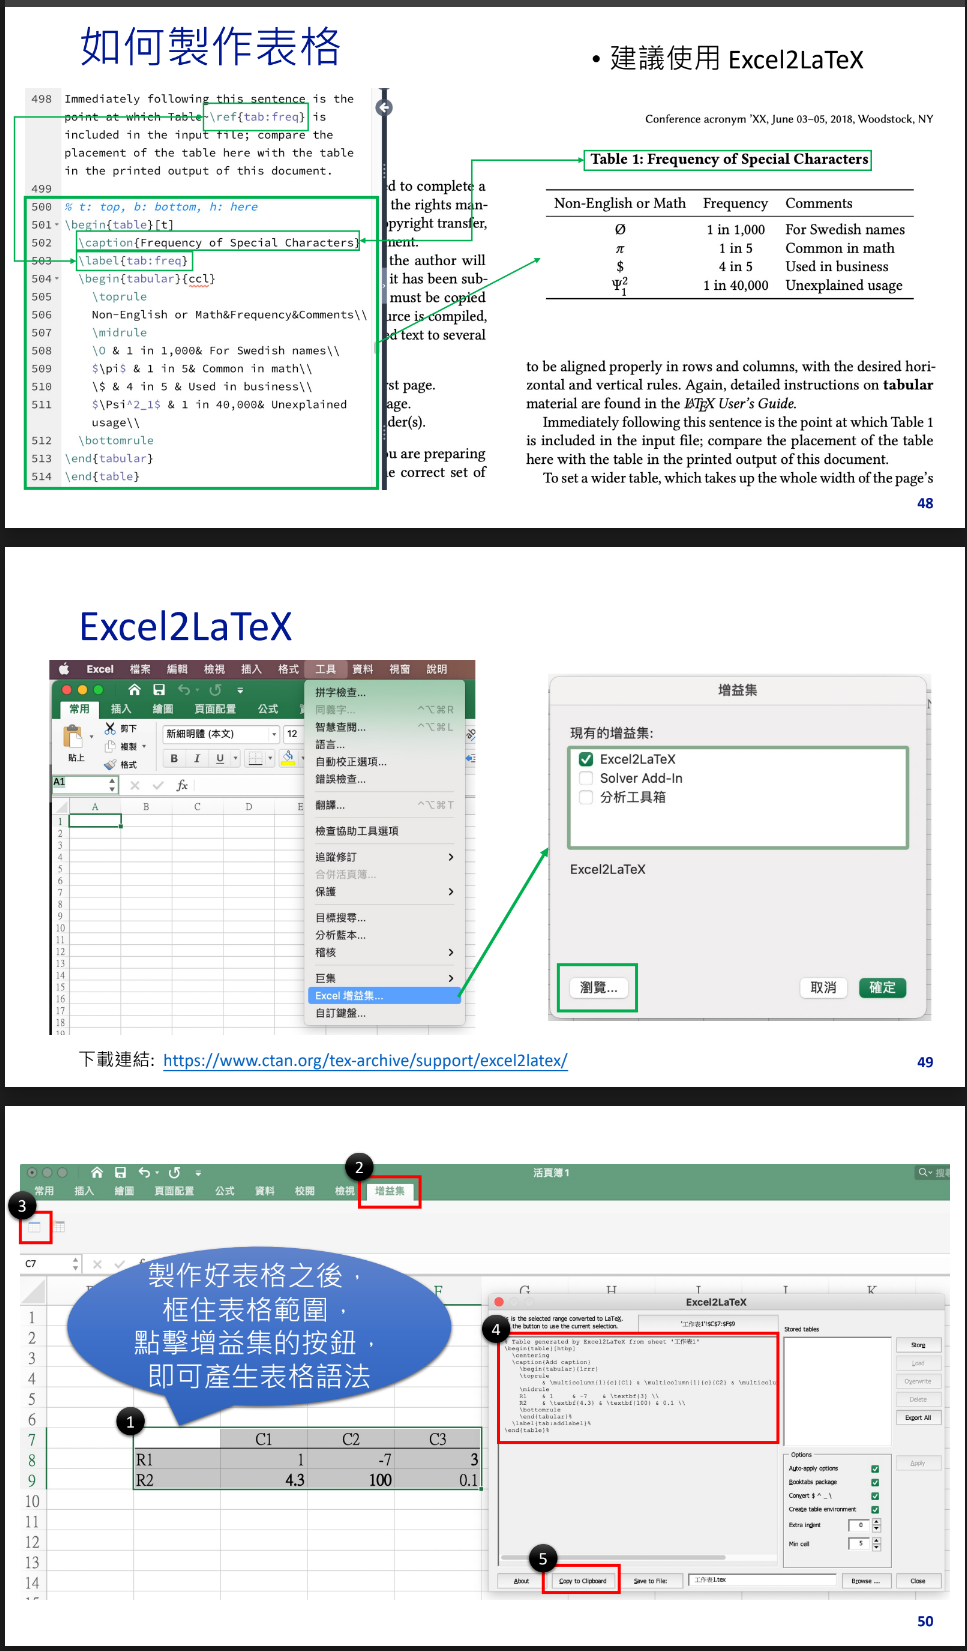
\includegraphics[width=0.8\textwidth]{img/excel2latex.png}
	\caption{Excel2LaTeX.}
	\label{fig:excel2latex}
\end{figure}

 \newpage
\chapter{Data Fusion Algorithm}
\label{ch:method}

\begin{figure}[htb]
	\centering
	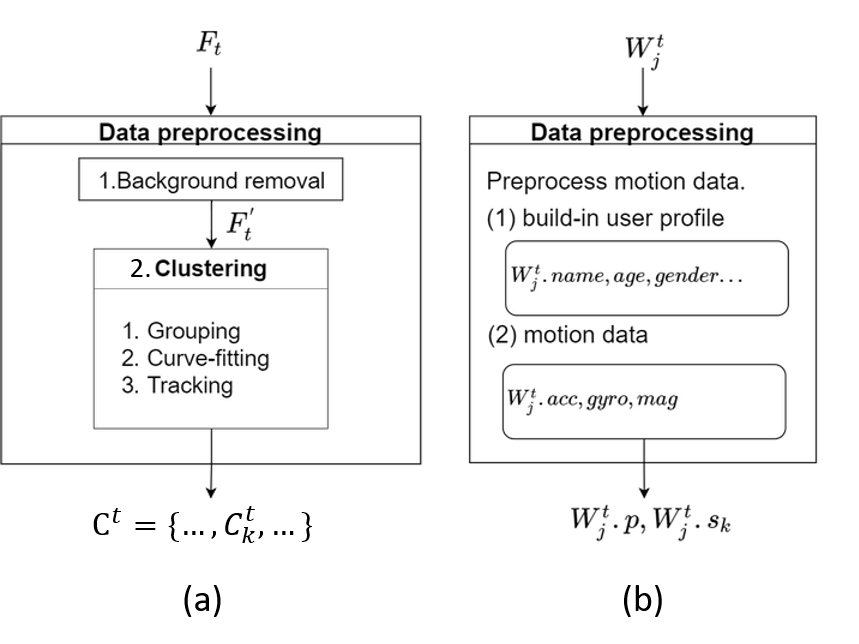
\includegraphics[width=0.6\textwidth]{img/data_preprocessing.png}
	\caption{An example for putting figure.}
	\label{fig:model}
	\vspace{-10mm}
\end{figure}

\section{Data Preprocessing}
\label{sec:SMA}
An example for section. Both LiDAR and wearable sensors will generate continuous data to our fusion server. Fig~\ref{fig:model} shows how these raw data are preprocessed. 


\subsection{2D LiDAR Data}
An example for subection. The LiDAR data preprocessing contains two parts: (i) background removal and (ii) clustering. Background removal 
....

 \newpage
\chapter{Performance Evaluation}
\label{ch:evaluation}

In this section, 整理效能評估.

下面是subfigure的範例 (其實我個人不常用這個語法, 我都直接在繪圖工具上把圖片整合在一起 XD)

\begin{figure}
     \centering
     \begin{subfigure}[]{0.3\textwidth}
         \centering
         
\includegraphics[width=\textwidth]{img/fig1.png}
         \caption{figure 1}
         \label{fig:11111}
     \end{subfigure}
     \hfill
     \begin{subfigure}[]{0.3\textwidth}
         \centering
         
\includegraphics[width=\textwidth]{img/fig2.png}
         \caption{figure 2}
         \label{fig:22222}
     \end{subfigure}
     \hfill
     \begin{subfigure}[]{0.3\textwidth}
         \centering
         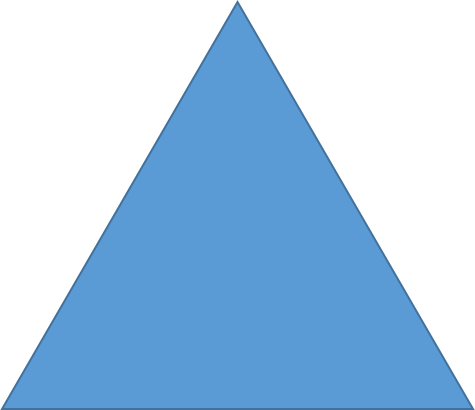
\includegraphics[width=\textwidth]{img/fig3.png}
         \caption{figure 3}
         \label{fig:33333}
     \end{subfigure}
        \caption{Three simple graphs}
        \label{fig:three graphs}
\end{figure} \newpage
\chapter{Conclusions}
\label{ch:conclusion}
Write your conclusion here.
 
 \newpage
% =========================================================================


% =========================================================================
% 參考文獻的檔案 Reference file: ref.bib
% ref的寫法可以參考這邊: https://hackmd.io/Bc1-FIIISka6DW15sPprAw
\ClearShipoutPicture % 把ref的浮水印關掉

\addcontentsline{toc}{chapter}{Bibliography}
\bibliographystyle{IEEEtran}
\bibliography{ref}
}
% =========================================================================


\end{CJK*}
\balance

\end{document}
